\documentclass{article}
\usepackage[a4paper]{geometry}
\usepackage[english]{babel}
\usepackage[utf8]{inputenc}
\usepackage{url}
\usepackage{hyperref}
\usepackage{graphicx}
\usepackage{amsmath}
\usepackage{amsfonts}
\usepackage{amssymb}
\usepackage{amsthm}
\usepackage{float}

\newcommand{\Sum}[3]{\ensuremath{\displaystyle\sum\limits_{#1}^{#2} #3}}

\title{Activity 4}
\author{Lucas Guesser Targino da Silva - RA: 203534}

\begin{document}

\section*{Problem Description}

Consider Cayley Trees $T(k, P)$ as defined in
\href{http://networksciencebook.com/chapter/3#homework3}{Problem 4 of Barabasi's book, Chapter 3 on Random Networks}, for $k >= 3$:

\begin{enumerate}
    \item Find a formula for the diameter $d_{\max}(k, P)$ of $T(k, P)$ in terms of $k$ and $P$.
    \item Find a formula for the number of vertices $N(k, P)$ of $T(k, P)$ in terms of $k$ and $P$.
    \item For a fixed $k$ which is different for each student (see below), plot a graph showing the values of $d_{\max}(k, P)$ and $\log(N(k, p))$, for $P$ ranging from $1$ to $10$.  Do you see a tendency as P grows?
\end{enumerate}

The attached table contains the values of $k$ to be used by each student.  Find your first two initials in the table and use the corresponding value of $k$.

\begin{table}[!ht]
    \centering
    \begin{tabular}{|c|c|}
        \hline
        student initials & k\\\hline\hline
        AI & 16 \\\hline
        FG & 3 \\\hline
        GO & 4 \\\hline
        LO & 5 \\\hline
        LG & 6 \\\hline
        IB & 7 \\\hline
        MA & 8 \\\hline
        MF & 9 \\\hline
        MM & 10 \\\hline
        MI & 11 \\\hline
        PH & 12 \\\hline
        RB & 13 \\\hline
        RC & 14 \\\hline
        VJ & 15 \\\hline
    \end{tabular}
    \caption{value of $k$ for each student.}
\end{table}

\section{Formula for the diameter}

\begin{quotation}
    maximum diameter $d_{\max}$: the maximum shortest path in the network
\end{quotation}

For a Cayley tree, $d_{\max}$ is the distance between two leaf vertices which are not in the same branch of the main vertex:

\begin{equation}
    d_{\max}(k, P) = 2 \cdot P = P + P
\end{equation}

the first $P$ is the distance from one leaf vertex to the root of the tree. The second is the distance to the target vertex (the other leaf vertex).

\section{Formula for the number of vertices}

\begin{enumerate}
    \item The level 0 has 1 vertex: the root of the tree.
    \item The level $l$ ($l \geq 1$) has $N_L(l, k)$ vertices:
        \begin{equation}
            N_L(l, k) = k \cdot {\left(k - 1\right)}^{l - 1}
        \end{equation}
    \item The total number of vertices is the sum of the number of vertices of each level up to the level $P$:
        \begin{equation}
            N(k,P) = \Sum{i = 0}{P}{N_L(l,k)} = 1 + k \cdot \dfrac{{\left(k - 1\right)}^{P} - 1}{k - 2}
        \end{equation}
\end{enumerate}

\section{Plot of the number of nodes and the diameter}

\begin{figure}[!ht]
    \centering
    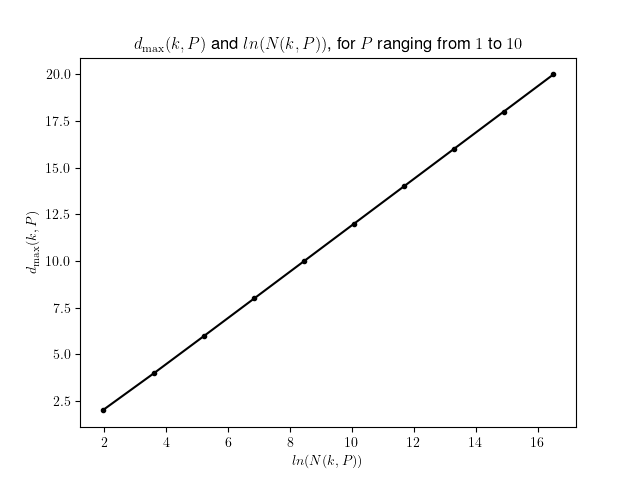
\includegraphics[width=0.7\textwidth]{../result/diameter_as_a_function_of_the_number_of_nodes.png}
    \caption{$d_{\max}(k, P)$ as a function of $ln{\left(N(k,P)\right)}$}
    \label{figure:plot}
\end{figure}

Notice that there is a clear exponential tendency in the Figure \ref{figure:plot}. One can describe the relation with the function:

\begin{equation}
    d_{\max}(N) = \alpha \cdot \ln(N) + \beta
\end{equation}

For the data used to produce the Figure \ref{figure:plot} ($k=6$, $P$ from 1 to 10), using curve fit, one finds the values:

\begin{enumerate}
    \item $\alpha = 1.2392486252985329 \pm 0.0015234289193245037$
    \item $\beta = -0.4615606209981668 \pm 0.015760537821112773$
\end{enumerate}


\end{document}
